\chapter{Van zaad tot plant}\label{ch:g2:from-seed-to-plant}

Schud een gedroogde bonenpeul en er rammelen harde boontjes uit ---
droog, saai, ogenschijnlijk net zo levenloos als grind. Maar \omterm{def:g1:plants-around-us:plant}{plant} er
één in de aarde en geef het water, en binnen een paar dagen gebeurt er
ondergronds iets buitengewoons. Er zat een hele \omterm{def:g1:plants-around-us:plant}{plant} opgevouwen in te
wachten op haar sein.

\section{Wat een zaad is}

\begin{definition}[Zaad]\label{def:g2:from-seed-to-plant:seed}
Een \emph{zaad}\index{zaad} is het begin van een nieuwe \omterm{def:g1:plants-around-us:plant}{plant}, gemaakt
door de moederplant. Binnen zijn beschermende schil bevat een zaad:
\begin{itemize}
  \item een piepklein plantje dat al begonnen is --- de
        \emph{kiem}\index{kiem} van de \omterm{def:g1:plants-around-us:plant}{plant}, met het begin van een
        \omterm{def:g1:plants-around-us:parts}{wortel} en een scheut;
  \item een voorraad voedsel om het te voeden tot het zichzelf kan voeden.
\end{itemize}
\end{definition}

\begin{example}[Een geweekte boon openen]\label{ex:g2:from-seed-to-plant:open}
Week een grote witte boon een nacht, en zijn schil glijdt er
gemakkelijk af. De boon valt uiteen in twee dikke helften --- de
voedselvoorraad --- en daar, tegen één rand aan genesteld, ligt een
piepklein bleek plantje, worteltip en opgevouwen eerste blaadjes, zo
klein als een rijstkorrel. Het nieuwe plantje zat er al die tijd al.
\end{example}

\begin{omfigure}
\begin{tikzpicture}
  \node[anchor=south west, inner sep=0] (img) at (0,0)
    {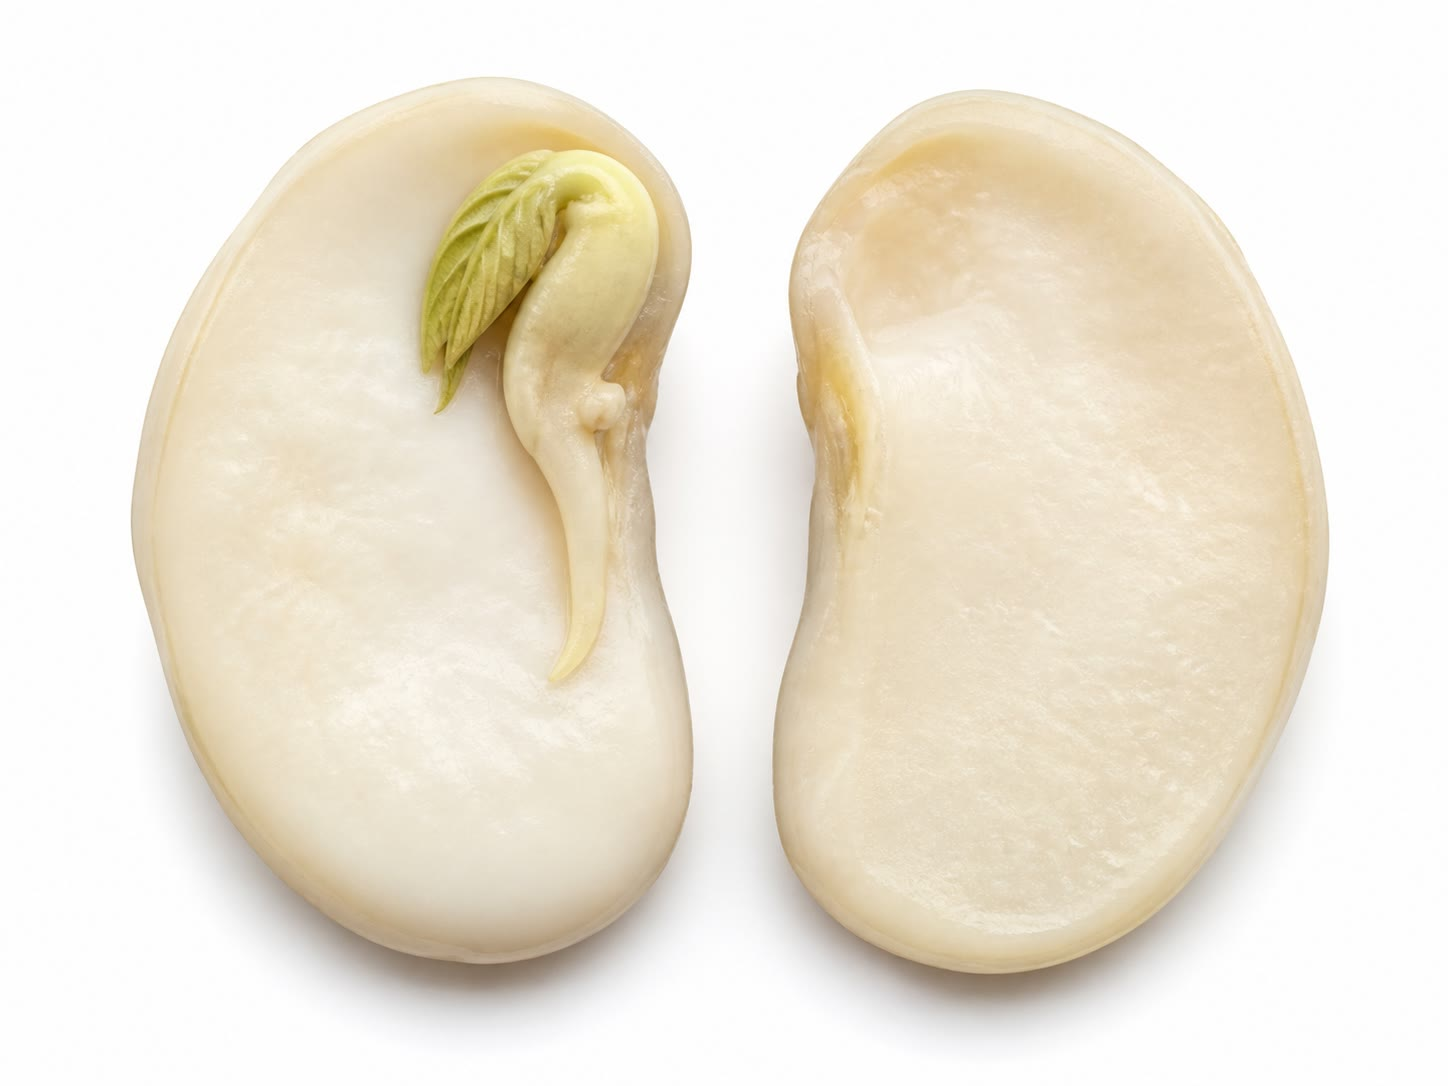
\includegraphics[width=0.62\linewidth]{images/book1/ai/fig-bean-open.jpg}};
  \begin{scope}[x={(img.south east)}, y={(img.north west)},
      every node/.style={font=\small}]
    \draw[omDef, thick] (0.35,0.79) -- (0.26,0.94)
      node[above] {de opgevouwen eerste blaadjes};
    \draw[omDef, thick] (0.40,0.38) -- (0.28,-0.04)
      node[below] {de worteltip};
    \draw[omDef, thick] (0.78,0.35) -- (0.80,-0.04)
      node[below, align=center] {de twee dikke helften:\\ de voedselvoorraad};
  \end{scope}
\end{tikzpicture}

{\small In de geweekte, geopende boon: een piepklein plantje ---
worteltip en opgevouwen eerste blaadjes --- tegen zijn voedselvoorraad aan.}
\end{omfigure}

\begin{remark}[Zaden reizen door onze keukens]\label{rem:g2:from-seed-to-plant:kitchen}
Bonen, erwten, linzen, rijst, zonnebloempitten, de pitjes in de appel
en de pit in de perzik: de keuken zit vol zaden. Sommige zijn
piepklein, zoals maanzaad; de kokosnoot is een reus. Elk van ze zou,
als het de kans kreeg, proberen een \omterm{def:g1:plants-around-us:plant}{plant} te worden.
\end{remark}

\section{Ontkiemen}

\begin{definition}[Ontkieming]\label{def:g2:from-seed-to-plant:germination}
\emph{Ontkieming}\index{ontkieming} is het moment waarop een \omterm{def:g2:from-seed-to-plant:seed}{zaad}
wakker wordt en begint te groeien: het zwelt op met water, zijn schil
splijt, het worteltje komt er als eerste uit en duikt omlaag, en dan
komt de scheut omhoog, die de eerste groene blaadjes naar het licht
draagt. We zeggen dat het \omterm{def:g2:from-seed-to-plant:seed}{zaad} \emph{ontkiemt}\index{ontkiemen}.
\end{definition}

\begin{proposition}[Wat een zaad nodig heeft om te ontkiemen]\label{prop:g2:from-seed-to-plant:needs}
Om te \omterm{def:g2:from-seed-to-plant:germination}{ontkiemen} heeft een \omterm{def:g2:from-seed-to-plant:seed}{zaad} \emph{water} en \emph{warmte} nodig.
Licht heeft het nog niet nodig: de voedselvoorraad voedt het
\omterm{prop:g2:from-seed-to-plant:cycle}{kiemplantje} in het begin, zelfs onder de grond, in het donker. Zonder
water, of in de kou, wacht een goed \omterm{def:g2:from-seed-to-plant:seed}{zaad} gewoon af.
\end{proposition}
\admitted

\begin{example}[Waarom je pas in de lente zaait]\label{ex:g2:from-seed-to-plant:spring}
Tuinders zaaien bonen in de lente, niet in de winter: het \omterm{def:g2:from-seed-to-plant:seed}{zaad} zou in
koude aarde blijven wachten --- of rotten --- in plaats van \omterm{def:g2:from-seed-to-plant:germination}{ontkiemen}.
Warme dagen en vochtige aarde zijn precies de twee seinen uit
\cref{prop:g2:from-seed-to-plant:needs}.
\end{example}

\begin{method}[Een zaad zaaien en zien ontkiemen]\label{met:g2:from-seed-to-plant:sow}
\begin{enumerate}
  \item Bekleed een glazen pot met vochtige watten of papier;
  \item schuif een boon tussen het glas en de watten, zodat je hem kunt zien;
  \item zet de pot in een warme kamer en houd de watten vochtig;
  \item kijk elke dag en schrijf op wat je ziet: opzwellen, de schil die
        splijt, \omterm{def:g1:plants-around-us:parts}{wortel} omlaag, scheut omhoog.
\end{enumerate}
Het glas maakt zichtbaar wat anders onder de grond gebeurt.
\end{method}

\begin{omfigure}
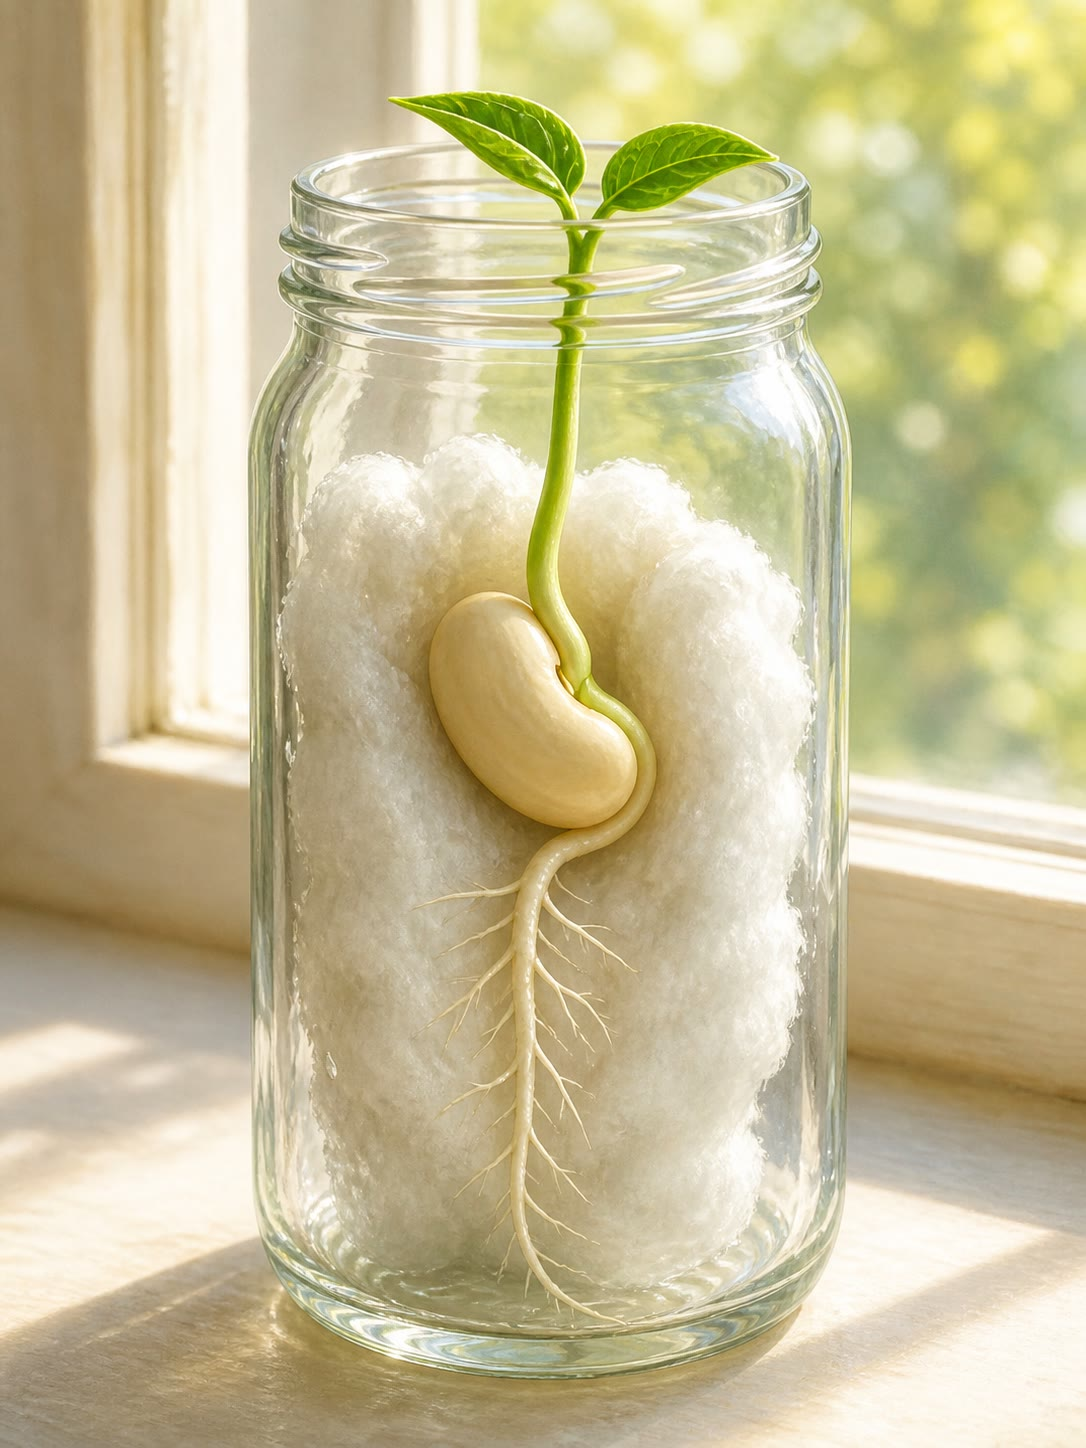
\includegraphics[width=0.44\linewidth]{images/book1/ai/g2-seed-bean-jar.jpg}

{\small De potproef midden in de \omterm{def:g2:from-seed-to-plant:germination}{ontkieming}: \omterm{def:g1:plants-around-us:parts}{wortel} omlaag, scheut
omhoog, en het leeglopende \omterm{def:g2:from-seed-to-plant:seed}{zaad} ertussen.}
\end{omfigure}

\begin{remark}[Wortel omlaag, scheut omhoog --- altijd]\label{rem:g2:from-seed-to-plant:updown}
Hoe de boon ook in de pot ligt --- op zijn kant, ondersteboven --- de
\omterm{def:g1:plants-around-us:parts}{wortel} draait altijd omlaag en de scheut altijd omhoog. Het
\omterm{prop:g2:from-seed-to-plant:cycle}{kiemplantje} kan niet zien, en toch weet het welke kant boven is.
\omterm{def:g1:plants-around-us:plant}{Planten} voelen meer dan ze laten zien.
\end{remark}

\section{Van kiemplantje tot plant met zaden}

\begin{proposition}[De levenscyclus van de plant]\label{prop:g2:from-seed-to-plant:cycle}
Het \emph{kiemplantje}\index{kiemplantje} groeit uit tot een \omterm{def:g1:plants-around-us:plant}{plant} met
\omterm{def:g1:plants-around-us:parts}{wortels}, \omterm{def:g1:plants-around-us:parts}{stengel} en \omterm{def:g1:plants-around-us:parts}{bladeren}; de \omterm{def:g1:plants-around-us:plant}{plant} bloeit; de \omterm{def:g1:plants-around-us:parts}{bloemen} maken nieuwe
\emph{zaden}; en de cyclus kan opnieuw beginnen. Eén bonenplant kan in
één zomer tientallen nieuwe bonen maken.
\end{proposition}
\admitted

\begin{example}[Eén boon, één zomer]\label{ex:g2:from-seed-to-plant:summer}
In mei gezaaid, \omterm{def:g2:from-seed-to-plant:germination}{ontkiemt} een boon binnen een week; in juni is het een
bladerrijke \omterm{def:g1:plants-around-us:plant}{plant} die tegen haar stok op klimt; in juli komen er witte
\omterm{def:g1:plants-around-us:parts}{bloemen}, dan groene peulen; in augustus hangen de peulen zwaar, elk met
een rij nieuwe bonen --- de zaden van volgend jaar, gemaakt door de
\omterm{def:g1:plants-around-us:plant}{plant} van dit jaar.
\end{example}

\section{Oefeningen}

\begin{exercise}[$\star$]\label{exo:g2:from-seed-to-plant:1}
Welke twee dingen liggen er binnen de schil van een \omterm{def:g2:from-seed-to-plant:seed}{zaad}?
\end{exercise}

\begin{exercise}[$\star$]\label{exo:g2:from-seed-to-plant:2}
Wat betekent \emph{\omterm{def:g2:from-seed-to-plant:germination}{ontkiemen}}? Wat komt er als eerste uit het \omterm{def:g2:from-seed-to-plant:seed}{zaad}: de
\omterm{def:g1:plants-around-us:parts}{wortel} of de scheut?
\end{exercise}

\begin{exercise}[$\star$]\label{exo:g2:from-seed-to-plant:3}
Noem de twee dingen die een \omterm{def:g2:from-seed-to-plant:seed}{zaad} nodig heeft om te \omterm{def:g2:from-seed-to-plant:germination}{ontkiemen}. Welke
beroemde behoefte van volgroeide \omterm{def:g1:plants-around-us:plant}{planten} staat \emph{niet} op de lijst?
\end{exercise}

\begin{exercise}[$\star$]\label{exo:g2:from-seed-to-plant:4}
Hoe kan een begraven \omterm{prop:g2:from-seed-to-plant:cycle}{kiemplantje} in het donker groeien, voordat het het
licht bereikt? Waar komt zijn voedsel in het begin vandaan?
\end{exercise}

\begin{exercise}[$\star$]\label{exo:g2:from-seed-to-plant:5}
Noem vier zaden die je in een keuken zou kunnen vinden.
\end{exercise}

\begin{exercise}[$\star$]\label{exo:g2:from-seed-to-plant:6}
Waarom zaaien tuinders in de lente en niet in de winter?
\end{exercise}

\begin{exercise}[$\star$]\label{exo:g2:from-seed-to-plant:7}
Zet op volgorde: peul met nieuwe bonen --- \omterm{def:g2:from-seed-to-plant:seed}{zaad} --- bloeiende \omterm{def:g1:plants-around-us:plant}{plant} ---
\omterm{prop:g2:from-seed-to-plant:cycle}{kiemplantje} --- bladerrijke \omterm{def:g1:plants-around-us:plant}{plant}.
\end{exercise}

\begin{exercise}[$\star$]\label{exo:g2:from-seed-to-plant:8}
Probeer het: zet de glazen pot van \cref{met:g2:from-seed-to-plant:sow}
op met twee bonen --- een op zijn kant, een ondersteboven. Vergelijk na
de \omterm{def:g2:from-seed-to-plant:germination}{ontkieming} hun \omterm{def:g1:plants-around-us:parts}{wortels} en hun scheuten. Wat voorspelt
\cref{rem:g2:from-seed-to-plant:updown}?
\end{exercise}

\begin{exercise}[$\star\star$]\label{exo:g2:from-seed-to-plant:9}
Nina bewaart een zakje bonenzaden een heel jaar in een droge la, en ze
\omterm{def:g2:from-seed-to-plant:germination}{ontkiemen} nog steeds als ze ze eindelijk zaait. Waarom zijn ze in de la
niet gegroeid en ook niet doodgegaan? Gebruik
\cref{prop:g2:from-seed-to-plant:needs}.
\end{exercise}

\begin{exercise}[$\star\star$]\label{exo:g2:from-seed-to-plant:10}
Het kuiken uit \cref{ch:g2:animals-grow-up} groeit in zijn \omterm{def:g2:animals-grow-up:born}{ei}, gevoed
door de dooier. Wat speelt de rol van de dooier in een boon? Wat hebben
een \omterm{def:g2:animals-grow-up:born}{ei} en een \omterm{def:g2:from-seed-to-plant:seed}{zaad} met elkaar gemeen?
\end{exercise}
